\section{全局线程池、重排序缓冲区与 Pipeline 聚合根}

前几章已经把数值内核（kernel）与 I/O 数据平面（data plane）拆开了；本章只讨论
\texttt{pipeline.cpp}。它不新增任何奇异值分解（Singular Value Decomposition, SVD）公式，
也不重新发明文件格式，而是负责把
\[
    \texttt{testcases}
    \longrightarrow
    \texttt{kernel}
    \longrightarrow
    \texttt{output}
\]
拼成一次端到端执行。换句话说，\texttt{JacobiSvdPipeline} 是应用层聚合根（aggregate root）：
它拥有调度权、关闭协议与错误传播语义，但不偷走 I/O 与 CUDA 内核的领域职责。

本章所讨论的并发骨架，采用一种以 \texttt{future} FIFO 队列实现的重排序缓冲区
（reorder buffer, ROB）。它把“乱序完成、顺序提交”这层语义折叠进一个
\textbf{按输入顺序排队的 \texttt{future} 队列}里。于是整体骨架可以写成
\[
    \texttt{input}
    \longrightarrow
    \texttt{dispatch}
    \longrightarrow
    \texttt{global thread pool}
    \longrightarrow
    \texttt{FIFO future queue}
    \longrightarrow
    \texttt{single writer}.
\]
如果借用处理器体系结构（computer architecture）的语言，这对应一个执行顺序与提交顺序分离、
并以有序提交（ordered commit）收敛结果的 ROB。
输入顺序必须保真，工作线程可以乱序完成，而文件输出必须回到确定性的提交顺序。
本章就围绕这层语义，展开 pipeline 的理论动机、控制流与工程边界。

\begin{center}
    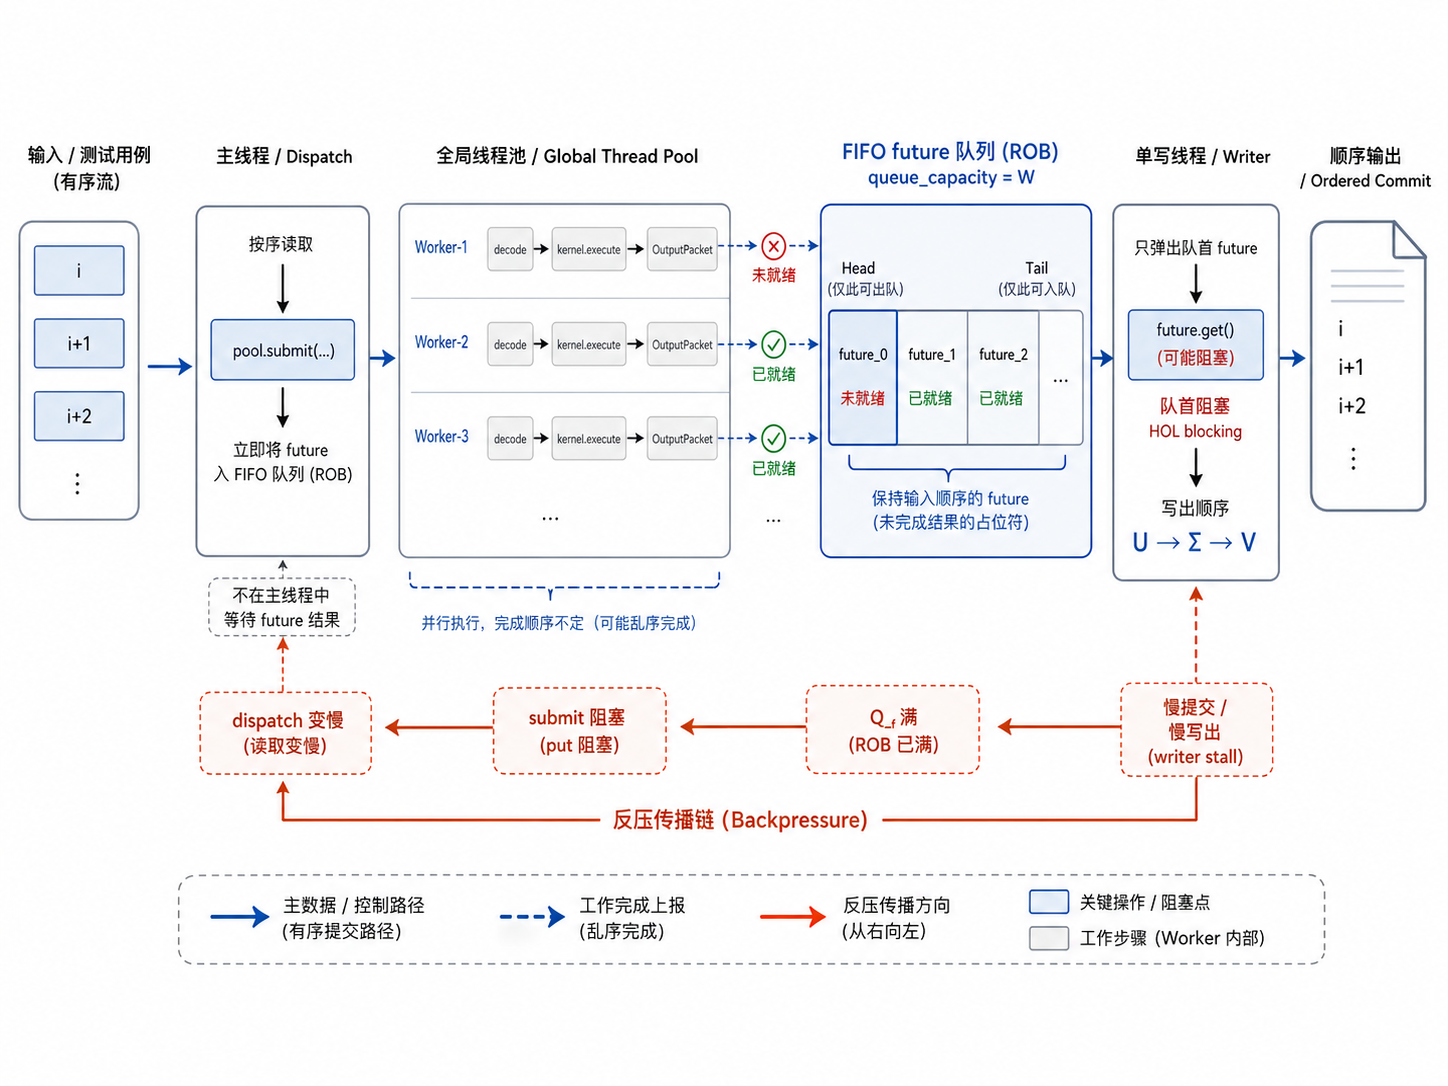
\includegraphics[width=0.92\textwidth]{figures/how-application-layer-works.png}
\end{center}

\subsection{为什么这样设计 pipeline：理论动机、顺序契约与复杂度边界}

先看最朴素的串行方案。若第 $i$ 个 testcase 的主要主机侧耗时分解为
\[
    R_i=\text{读取/派发},\qquad
    D_i=\text{解码},\qquad
    C_i=\text{SVD 计算},\qquad
    W_i=\text{写出},
\]
那么串行总耗时近似为
\[
    T_{\mathrm{serial}}
    =
    \sum_{i=0}^{N-1}(R_i+D_i+C_i+W_i).
\]
这种写法最容易理解，但它把文件读取、页锁定缓冲准备、GPU 计算与结果落盘全部压在一条长临界路径
（critical path）上。只要某一张矩阵稍慢，后面所有 testcase 都会被迫等待。

当前 pipeline 的思路不是在主机侧“暴力多线程化一切”，而是只把真正可并行的
\emph{跨 testcase 工作}交给全局线程池（global thread pool），并保留一个单线程 writer 负责稳定输出。
于是稳定阶段的端到端节拍更接近
\[
    T_{\mathrm{steady}}
    \approx
    \max(T_{\mathrm{dispatch}},T_{\mathrm{workers}},T_{\mathrm{commit}}),
\]
其中最后一项的名字特意写成 \texttt{commit} 而不是 \texttt{write}，
因为写线程当前做的不只是“把字节写出去”，它还承担了一个更强的顺序承诺：
\textbf{只有排在最前面的 future 可以提交，后面的结果即使先算完，也不能越过它。}

这就引出了顺序契约（ordering contract）。输入流天然有序：
\[
    X_0,X_1,\ldots,X_{N-1}.
\]
工作线程一旦并发执行，真实完成顺序就会变成某个排列
\[
    P_{\pi(0)},P_{\pi(1)},\ldots,P_{\pi(N-1)}.
\]
系统采用如下顺序契约：
\textbf{主线程按照输入顺序，把 \texttt{future<OutputPacket>} 依次送进输出阶段；写线程也按这一顺序依次取 future，
    并在提交点调用 \texttt{future.get()}。}
因此真正被提交到文件中的顺序不是“谁先算完”，而是
\[
    \texttt{commit}(0)
    \prec
    \texttt{commit}(1)
    \prec
    \cdots
    \prec
    \texttt{commit}(N-1).
\]
这一定义下，ROB 不通过显式散列表维护“谁已经完成但不能提交”的状态，
而是用队列顺序天然表达“谁有资格先提交”。

当然，这种 ROB 设计也不是免费午餐。它把原本的“显式按 index 回填复杂度”换成了“队首阻塞
（head-of-line blocking）”。若 future$_0$ 迟迟不完成，而 future$_1$、future$_2$ 已经 ready，
写线程仍然必须在
\[
    \texttt{future}_0.\texttt{get()}
\]
处等待。这意味着当前实现优化的是\textbf{状态简洁性与顺序确定性}，而不是“谁先完成谁先提交”的最大化吞吐。
对本项目来说，这是一个很合理的工程取舍：实验结果的稳定顺序比额外引入一套乱序完成表更重要。

第三个约束是内存与 in-flight 上界。CLI 把 \texttt{--queue-capacity} 解释为
\[
    W=\max(\texttt{max\_queued\_results},1).
\]
但必须精确说明：这里的 $W$ 直接限制的是
\texttt{FutureQueueOutputStage} 内部 \texttt{future\_queue\_} 的容量，而不是“所有尚未写出的对象总数”的严格数学上界。
这是因为 writer 线程会先把一个 future 从队列里弹出，再在队列外执行 \texttt{get()}；
主线程也可能在 \texttt{submit()} 被阻塞前，刚刚多提交了一个对应 worker 任务。于是更准确的说法是：
\[
    M_{\mathrm{pending}}
    =
    O((W+\delta)\cdot E_{\max}),
\]
其中 $E_{\max}$ 表示单个 testcase 结果包的最大规模，
$\delta$ 是由“writer 手中正在等待的一个 future”和“生产者临界区外的一次过渡提交”引入的小常数。
这不是 profiling 精确值，而是一条更诚实的系统结论：系统仍然是\emph{有界}的，但边界来自
``有界 future admission''。

最后一个约束是错误诚实性（error honesty）。并发系统最怕的不是抛异常本身，
而是某个线程已经知道结果不可信，而主线程还在继续把流程包装成“成功执行完毕”。
本章后面的所有细节，无论是关闭协议、原子计数、还是 writer 线程统一吸收 future 异常，
本质上都服务于同一个目标：\textbf{一旦任一阶段认定结果不再可信，\texttt{run()} 最终就不能报告成功。}

\subsection{全局线程池实现：把并发入口集中起来，而不是到处偷开线程}

\texttt{GlobalThreadPool} 依然刻意保持极小语义集合。它是一个惰性初始化
（lazy initialization）的进程内全局对象：
\[
    \texttt{global\_thread\_pool()}
    \Rightarrow
    \texttt{static GlobalThreadPool pool(default\_thread\_pool\_size())}.
\]
默认线程数来自 \texttt{std::thread::hardware\_concurrency()}，若运行环境不给出可信值，则回退到 $4$。
构造时一次性创建 worker；析构时设置 \texttt{stopping\_}，唤醒所有线程，再逐个 \texttt{join()}。

它的工作线程主循环几乎可以压缩成三步：
\[
    \text{wait until } \texttt{stopping\_}\lor\neg Q.empty()
    \longrightarrow
    \text{pop one task}
    \longrightarrow
    \text{execute outside lock}.
\]
这里最重要的好品味（good taste）不是“用了线程池”这件事本身，
而是线程池\textbf{不理解业务顺序语义}。它只知道自己维护
\texttt{std::queue<std::function<void()>>}，
并通过条件变量（condition variable）协调 worker 睡眠与唤醒。
至于 testcase 是第几号、输出该不该有序、某个 future 何时能提交，都不属于线程池的职责。

\texttt{submit()} 返回的不是
\texttt{std::future<void>}，而是模板化的
\[
    \texttt{std::future<ResultType>}.
\]
具体做法是把调用者传入的可调用对象（callable）包装成
\texttt{std::packaged\_task<ResultType()>}，再把该 task 的执行闭包压入线程池队列。
这有两个直接收益。

\begin{itemize}
    \item 线程池不需要知道结果类型是什么；它只执行闭包，不解释 \texttt{OutputPacket}。
    \item worker 里抛出的异常会自动落入 future 的共享状态（shared state），后续由 writer 线程在
          \texttt{future.get()} 处统一观察。
\end{itemize}

这点很关键，因为当前实现已经把“错误汇聚点”从主线程转移到了输出阶段。
主线程提交给线程池的闭包通常长成下面这种形式：
\[
    \texttt{task}
    \longrightarrow
    \texttt{decode}
    \longrightarrow
    \texttt{kernel.execute}
    \longrightarrow
    \texttt{return OutputPacket}.
\]
线程池只负责把这个函数跑完；它既不会主动 \texttt{get()} 结果，也不会替 pipeline 写文件。

为什么线程池继续保留为全局对象，而不是每次 \texttt{run()} 都新建一批线程？
核心原因仍然有三点：

\begin{itemize}
    \item 线程创建与销毁不是零成本；
    \item 并发总量需要有集中入口，否则每层各自“只多开一点点线程”很快就会失控；
    \item pipeline 是应用层协议，不应重复建造同一种宿主基础设施。
\end{itemize}

当然，也要诚实指出它的边界。当前线程池内部任务队列本身并\textbf{没有}容量上界，
真正的背压主要来自外层的 \texttt{FutureQueueOutputStage::submit()}。
这意味着：只要所有任务都遵循“提交一个 worker future 后立刻尝试送入输出阶段”的当前控制流，
系统的 in-flight 数量就是有限的；但如果未来有别的模块直接复用这同一个全局线程池并大量投递任务，
那就需要重新讨论 bounded queue、独立执行器（executor）或更细的资源隔离。

\subsection{流程与重排序缓冲区：主线程派发、工作线程执行、写线程恢复顺序}

这一节讨论的重排序缓冲区，是“按输入顺序排队的 future 提交队列 + 单 writer 顺序 \texttt{get()}”。
从抽象效果看，它实现的是 ordered commit；从实现形态看，它是一个 FIFO future-queue ROB。

从控制流看，\texttt{run()} 的主骨架现在更接近下面这条链：
\[
    \begin{aligned}
        \text{normalize config}
         & \longrightarrow
        \text{read testcase } i
        \longrightarrow
        \text{submit worker future}    \\
         & \longrightarrow
        \text{enqueue future in FIFO output stage}
        \longrightarrow
        \text{writer pops next future} \\
         & \longrightarrow
        \texttt{future.get()}
        \longrightarrow
        \text{write } U_i,\Sigma_i,V_i.
    \end{aligned}
\]
这里最值得注意的一点是：\textbf{输出阶段接收的不是已经完成的 \texttt{OutputPacket}，而是
    未来会产生该 packet 的 \texttt{future}}。因此“消费者”其实消费的是\emph{提交资格}，而不是现成结果。

\paragraph{第一步：主线程保留单游标读取权。}
对于 \texttt{*.mat} 路径，\texttt{io::MatDispatchReader} 顺序读出
\texttt{MatDispatchTask}。该对象里已经带有
\[
    (\texttt{sequence\_index},\texttt{rows},\texttt{columns},\texttt{buffer})
\]
这组信息，其中 \texttt{buffer} 是由 \texttt{cudaMallocHost} 管理的页锁定主机内存
（page-locked host memory, pinned host memory）。
主线程每次把读出的 dispatch task 移动到局部对象 \texttt{task\_for\_worker}，
随后立刻把原变量重置为空任务，以保持所有权边界清晰。

对于 \texttt{*.txt} 路径，则由 \texttt{TextTestcaseSource} 在主线程中直接解析出
\texttt{io::Matrix}，再把该矩阵移动给 worker。也就是说，当前实现把
\texttt{*.mat} 与 \texttt{*.txt} 的差异放在“任务准备形态”这一层，而不是强行让二者共享一套低层数据结构。

\paragraph{第二步：worker 闭包只负责单 testcase 的局部工作。}
两条输入路径最终都归约到同一件事：提交一个返回 \texttt{OutputPacket} 的闭包。
在 \texttt{*.mat} 路径里，闭包会先执行
\[
    \texttt{io::decode\_dispatch\_task\_matrix(task)},
\]
把网络字节序载荷解码为 \texttt{io::Matrix}；在 \texttt{*.txt} 路径里，这一步已经提前在主线程完成。
随后两条路径都调用
\[
    \texttt{kernel.execute(testcase, testcase\_index)},
\]
其中 \texttt{KernelStage::execute()} 先检查
\[
    rows>0,\qquad columns>0,\qquad |\texttt{values}|=rows\cdot columns,
\]
再调用 \texttt{one\_sided\_jacobi\_svd()}，
最后把结果组织成
\[
    P_i=(i,s_i,U_i,\Sigma_i,V_i).
\]
这里的 \texttt{testcase\_index} 仍然被保存在 \texttt{OutputPacket} 里，
但 writer \textbf{并不依赖该 index 做重排}；它更像一种审计字段（audit field）与调试字段。

\paragraph{第三步：future 在生成后立刻进入输出阶段，而不是先在主线程积压。}
\texttt{run()} 并没有维护额外的
\texttt{inflight deque}。相反，主线程在每次
\[
    \texttt{pool.submit(...)} \longrightarrow \texttt{future<OutputPacket>}
\]
之后，会立即执行
\[
    \texttt{output.submit(std::move(packet\_future))}.
\]
因此，主线程不手工轮询一串 future 来决定“哪一个先 ready”，而是把这个顺序资格整体转交给输出阶段。
这让主线程的责任进一步收缩成“顺序读取、顺序投递”。

\paragraph{第四步：\texttt{FutureQueueOutputStage} 用 FIFO future 队列表达 ROB 的 ordered commit。}
输出阶段内部最核心的状态不是“已完成 packet 映射表”，而是
\[
    Q_f=\texttt{future\_queue\_}.
\]
\texttt{submit()} 的协议是：只有当
\[
    |Q_f|<\texttt{queue\_capacity\_}
    \quad\lor\quad
    \texttt{closed\_}
    \quad\lor\quad
    \texttt{worker\_error\_}\neq\varnothing
\]
时，生产者线程才能继续。否则主线程会在条件变量上等待。
一旦 admission 成功，该 future 就按输入顺序被压入 FIFO 队列。

writer 线程的主循环则执行另一条极简状态机：
\[
    \text{pop front future}
    \longrightarrow
    \texttt{future.get()}
    \longrightarrow
    \texttt{write\_packet(packet)}
    \longrightarrow
    \texttt{written\_count\_++}.
\]
\texttt{ResultWriter::write\_packet()} 又进一步固定了每个 testcase 的落盘顺序：
\[
    U_i \longrightarrow \Sigma_i \longrightarrow V_i.
\]
所以，这个 ROB 的“顺序恢复”不是通过比较 \texttt{packet.testcase\_index} 完成的，
而是通过\textbf{谁先被压入 future 队列，谁就先拥有提交资格}来完成的。

\paragraph{第五步：队首阻塞是显式接受的系统属性。}
由于 writer 会在拿到队首 future 后直接调用 \texttt{get()}，所以它天然具备以下性质：
\[
    \text{if }\texttt{future}_i\text{ not ready, then commit}_{i+1}\text{ cannot happen.}
\]
换句话说，后面的 testcase 即使已经算完，也不能越过更早的 testcase 提交。
这说明系统采用的是\emph{有序提交窗口}，而不是“谁先完成谁先提交”的策略。

这套机制的好处是状态少、推理简单、错误路径更短。坏处也同样真实：一旦某个早期 testcase 特别慢，
writer 就会在它前面卡住，后续 ready 的结果只能在 future 共享状态中等待。
所以这里不存在所谓“纯优势升级”；它是一个非常典型的 systems trade-off：
\textbf{用更小的协议状态，换取可接受的 head-of-line blocking。}

\paragraph{第六步：背压沿着生产者-消费者链条自动回传。}
一旦 writer 比较慢，或者某个队首 future 长时间不 ready，
\texttt{future\_queue\_} 就会逐步占满。此时主线程会在 \texttt{output.submit()} 处阻塞，
从而形成如下背压链：
\[
    \text{slow commit or slow writer}
    \rightarrow
    Q_f \text{ full}
    \rightarrow
    \text{producer blocked in submit}
    \rightarrow
    \text{dispatch slows down}.
\]
这条回路很重要，因为它意味着慢写出不会被伪装成“只是多用了一点内存”。
当前实现明确选择让吞吐退化显式发生，而不是让资源占用隐式膨胀。

\subsection{工程健壮性细节：配置归一化、关闭协议、异常传播与不变量}

并发骨架搭好之后，真正决定工程可用性的，是这些“看起来不起眼、但实际上最容易埋雷”的细节。
当前 \texttt{pipeline.cpp} 的健壮性，主要建立在四组机制上。

\paragraph{其一，先归一化配置，再启动并发。}
\texttt{run()} 一开始就检查输入/输出路径是否为空，再通过
\texttt{resolve\_file\_format()} 把 \texttt{auto\_detect} 解析成 \texttt{mat} 或 \texttt{txt}。
若用户启用了布局转置自动调优（layout-transpose auto-tuning），并且模式仍是
\texttt{LayoutTransposeMode::auto\_select}，pipeline 会先调用
\texttt{auto\_tune\_layout\_transpose\_threshold()}，
把推荐阈值写回本次运行使用的 \texttt{runtime\_kernel\_config}，
然后把 \texttt{layout\_transpose\_auto\_tune} 关掉。

这一步必须发生在任何 worker 启动之前。否则多个线程若各自拿着“尚未定型”的配置去 benchmark，
那同一次运行内部就会出现语义竞争（semantic race）：大家计算的并不是同一个程序。

\paragraph{其二，成功关闭与失败关闭是两条不同协议。}
成功路径上，主线程读完整个输入流后调用
\[
    \texttt{output.close\_success(submitted\_count)}.
\]
这会设置
\[
    \texttt{expected\_count\_}=submitted\_count,\qquad
    \texttt{closed\_}=true,
\]
唤醒等待中的线程，随后 \texttt{join()} writer 线程。
writer 结束后，系统还会额外检查
\[
    \texttt{written\_count\_}=\texttt{expected\_count\_}.
\]
若不相等，就直接抛错，而不是把缺包输出误判为成功。

失败路径上，任意主线程异常都会进入 \texttt{run()} 的外层 \texttt{catch}，
随后调用
\[
    \texttt{output.close\_error(std::current\_exception())}.
\]
这会把首个错误保存到 \texttt{worker\_error\_}，同时设置
\[
    \texttt{closed\_}=true,\qquad \texttt{abort\_}=true,
\]
再唤醒所有等待者并尝试回收 writer 线程。
也就是说，\textbf{关闭协议不是“一个 bool 完事”，而是明确区分 success close 与 error close。}

\paragraph{其三，异常传播的汇聚点已经转移到输出阶段。}
这一点与旧文档最不一样。当前 worker 任务抛出的异常，并不是由主线程直接 \texttt{future.get()} 观察到的，
而是由 writer 线程在
\[
    \texttt{future\_packet.get()}
\]
处统一观察。无论异常来自 dispatch task 解码失败、矩阵布局校验失败、SVD kernel 抛错，
还是 worker 闭包内部的任何其他异常，它们都会先进入 future 共享状态，
然后在 writer 线程被重新抛出。随后 \texttt{consumer\_main()} 的总 \texttt{catch(...)} 会把该异常保存到
\texttt{worker\_error\_} 中，并设置关闭/中止标志。

writer 自己的 I/O 异常同样走这条路径。例如目录创建失败、输出流构造失败、\texttt{write\_packet()} 失败、
\texttt{flush()} 失败，最后也都会变成
\[
    \texttt{worker\_error\_} \neq \varnothing.
\]
之后，主线程在后续 \texttt{submit()}、\texttt{close\_success()} 或 \texttt{close\_error()} 中都会被重抛。
于是异常传播图更接近：
\[
    \begin{aligned}
        \text{worker failure}
         & \rightarrow
        \texttt{future shared state}
        \rightarrow
        \texttt{writer thread get()} \\
         & \rightarrow
        \texttt{worker\_error\_}
        \rightarrow
        \texttt{submit/close rethrow}
        \rightarrow
        \texttt{run fails},
    \end{aligned}
\]
\[
    \text{writer failure}
    \rightarrow
    \texttt{worker\_error\_}
    \rightarrow
    \texttt{run fails}.
\]
这比“主线程自己轮询每个 future”更集中，也更符合当前有序提交模型。

\paragraph{其四，RAII 保证资源回收，显式协议保证语义诚实。}
\texttt{GlobalThreadPool} 的析构负责停止并 \texttt{join()} 工作线程；
\texttt{FutureQueueOutputStage} 的析构则调用 \texttt{close\_noexcept()} 作为兜底，
即使调用者忘记显式关闭，也尽量避免资源泄漏或悬挂线程。
但这里必须区分两种责任：

\begin{itemize}
    \item RAII（Resource Acquisition Is Initialization）负责“不要泄漏资源”。
    \item \texttt{close\_success()} / \texttt{close\_error()} 负责“不要伪造成功语义”。
\end{itemize}

也正因为如此，析构函数里的兜底关闭选择了 \texttt{noexcept} 吃掉异常；
真正应该向上报告的错误，必须出现在显式关闭路径中，而不是留给栈展开
（stack unwinding）去碰运气。

\paragraph{其五，不变量比技巧更重要。}
当前实现真正依赖的不变量（invariants）其实并不多，但每一条都很硬：

\begin{itemize}
    \item 主线程按输入顺序生成并提交 future；
    \item 每个成功 worker 恰好返回一个 \texttt{OutputPacket}；
    \item writer 只按 FIFO 顺序消费 future，不做额外排序；
    \item 每个 testcase 固定写出三张矩阵：$U/\Sigma/V$；
    \item \texttt{total\_sweeps} 只用于聚合统计，因此使用 \texttt{memory\_order\_relaxed} 即可；
    \item 任意线程感知到的不可信状态，最终都必须让 \texttt{run()} 失败。
\end{itemize}

并发代码最危险的地方，往往不是锁多不多，而是状态与例外太多。当前实现能保持可分析性，
正是因为它把关键状态压缩成了：一个全局线程池、一个有界 future 队列、一个 writer 线程、
一组关闭标志和一个异常指针。状态空间越小，正确性才越容易被真正推理，而不是靠祈祷。

\subsection{当前实现的边界与可演化方向}

在这套 future-queue 并发模型下，\texttt{pipeline.cpp} 的边界也相当清晰。
这些边界不是“将来一定要修”的 bug 列表，
更像是后续演化时必须显式作答的设计问题。

\paragraph{第一，\texttt{queue\_capacity} 限制的是 output-stage admission，而不是线程池内部队列。}
当前主线程的确会在每次生成 future 后立刻尝试 \texttt{output.submit()}，
因此系统不会无限制地向前推进；但线程池内部的 \texttt{queue\_} 仍然是无界的。
换句话说，当前资源控制依赖的是“外层控制流很克制”，而不是“底层执行器自带硬上限”。
如果未来还有别的模块复用这同一个全局线程池，现有的资源边界分析就需要重新做。

\paragraph{第二，ROB 的 ordered commit 天然带来 head-of-line blocking。}
当前设计最大优点是顺序语义清爽，最大代价也是顺序语义太清爽：
一旦较早的 testcase 明显更慢，writer 就必须在它的 future 上等待，
后面已经 ready 的 packet 不能越过它。若未来 profiling 表明这类阻塞成为关键瓶颈，
那才值得考虑改写成显式完成包缓存、按 index 提交的另一种 ROB 形式。
但那会立刻把状态机重新变复杂，因此不应在没有证据时过早优化。

\paragraph{第三，主机侧并发不等于设备侧并发。}
多个 worker 线程可以同时调用 \texttt{one\_sided\_jacobi\_svd()}，
但这并不自动意味着 GPU 上就会出现理想的 kernel 重叠
（kernel overlap）。设备端是否真正并行，仍取决于 CUDA runtime、stream 使用方式、
显存压力和底层硬件资源。当前 pipeline 优化的是\textbf{端到端任务组织}，
而不是承诺单 GPU 上一定存在某种特定重叠模式。

\paragraph{第四，\texttt{*.txt} 路径仍然把解析留在主线程。}
这让文本输入的错误定位和控制流都更简单，也更符合“文本是兼容路径而不是高吞吐路径”的定位。
但它同时意味着：若输入瓶颈发生在文本解析上，当前并发模型并不会替你 magically 消除它。
未来若真要并行化文本路径，需要单独设计解析任务边界，而不是把当前 \texttt{TextTestcaseSource} 机械丢进线程池。

\paragraph{第五，\texttt{OutputPacket::testcase\_index} 目前更多是元数据，而不是提交控制键。}
这里值得记一笔：index 只是“这个 packet 对应谁”的事实记录，而不是 writer 的排序依据。
如果将来有人看到该字段就自然假设“writer 靠它排序”，那就会读错代码。

\paragraph{第六，当前报告仍然偏向语义摘要，而不是完整遥测。}
\texttt{PipelineReport} 会返回 testcase 数、已写矩阵数、总 sweep 数以及布局转置运行时配置；
但它还不告诉我们 writer 在多少次 \texttt{future.get()} 上发生了明显等待，
也不告诉我们 future 队列的峰值占用和队首阻塞持续时间。
如果未来要严肃研究 pipeline 吞吐瓶颈，更合理的方向是增加 profiling/telemetry 结构，
而不是继续把 \texttt{PipelineReport} 膨胀成调试日志容器。

\paragraph{第七，当前失败语义仍然是保守的 fail-fast。}
一旦 reader、worker 或 writer 任一环节确认失败，整次 \texttt{run()} 都会被判定为失败。
系统不会尝试“跳过坏 testcase，继续写后面的好结果”，也不会承诺部分输出文件具有某种恢复协议
（recovery protocol）。这种选择有利于实验结果的可审计性，但若未来要支持部分恢复、断点续跑或按 testcase 容错，
就必须同步重写输出格式、报告语义与关闭协议。

\subsection{小结}

本章把 \texttt{pipeline.cpp} 重新定位为应用层聚合根（aggregate root）：它既不实现底层 I/O，
也不参与单矩阵 SVD 的数值推导，而是负责把顺序输入、并发计算与确定性输出组合成一个可验证的执行协议。
这一协议的关键不在于“线程更多了”，而在于\textbf{重排序缓冲区被表达为按输入顺序提交的 future 队列}：
writer 在固定提交点上执行 \texttt{future.get()}，由此实现 ROB 的 ordered commit。

因此，这一章真正的重点并不在于几个类名，而在于新的并发模型如何平衡三件事：
较高吞吐、稳定输出顺序和失败语义的诚实传播。它用全局线程池集中 host 侧并发，
用有界 future admission 施加背压，用单 writer 保证文件顺序，
再用显式关闭协议把所有线程中的异常收拢回 \texttt{run()}。
从 systems 角度看，这是一种更收缩、也更容易推理的设计；代价则是明确接受队首阻塞。
这份取舍本身，就是当前 \texttt{pipeline.cpp} 的核心思想。
